\documentclass[]{article}


\usepackage{graphicx}
\usepackage{fullpage}
\usepackage{appendix}
\usepackage{microtype}
\usepackage{mathtools,amssymb,amsthm,mathrsfs}

%opening
\title{Monte Carlo Simulations of Magnetic Systems}
\author{Jenny Poulton}

\begin{document}

\maketitle

This document illustrates the new data found from analysing the spin one triangular antiferromagnet using Glauber and Kawasaki dynamics and examines the dependence of the probabilities on spin for the square antiferromagnet using Kawasaki dynamics.

\section{Probabilities in Kawasaki Dynamics}

The general result for probabilities at high temperature using Kawasaki dynamics can be found by analysing the different types of pair systems which arise. This can be easily illustrated using the spin one system. There are 7 types of pairs which are able to flip using Kawasaki dynamics, 01, 10 and 0-1, -10 which can only convert into it's opposite leaving probabilities unchanged, and 1-1, -11 and 00 which lead to changes in probability.

We can relate $P_{00}$ and $P_{1-1}$/$P_{-11}$ together by looking at the possible flips for each pair.

\begin{align}
(1-1)& \rightarrow (00)\\
(-11)& \rightarrow (00)\\
(00)&\rightarrow
\begin{cases}
(1-1) \quad P=0.5\\
(-11) \quad P=0.5
\end{cases}
\end{align}

This tells us that the rate of change of pair type for$(1-1)$ and equivalently$(-11)$ is the number of this type of pair being removed which is all of the pairs of it's type being changed, subtracted from the number of this type of pair being added, which in this case is half the number of (00) pairs being changed. Similiarly for the rate of change of probability for $(00)$ pairs is the number of this type of pair being removed subtracted from the the number of them being added, which is the sum of the $(1-1)$ and the $(-11)$ pairs being changed. As the number of pairs of each type being changed is directly proportional to the probability of each type occuring it can be said that.

\begin{align}
\frac{d}{dt} P_{00} &= \alpha[-P_{00} + P_{-11} + P_{1-1}]\\
\frac{d}{dt} P_{1-1} &= \alpha[-P_{1-1} +\frac{1}{2}P_{00}]
\end{align}

Which both go to zero at equilibrium. By setting them equal to each other it can quickly be seen that $P_{1-1}=P_{-11}$ and $P_{00} = P_{1-1}$. We know that the probability of having a pair of adjacent particles with a specific value$P_{ab}$ is the product of the probabilities that the individual particles have the values a and b ($p_{a}$ and $p_{b}$). Thus;

\begin{align}
P_{00} &= p_{0}^{2} \\
P_{1-1} &= P_{-11} = p_{1}p_{-1} = p_{1}^2
\quad\quad (p_{1}=p_{-1})
\end{align}

Combining these tells us that $p_{0} = \sqrt{2}p_{\pm1}$. Normalising this gives $p_{\pm1} = 0.293$ and $p_{1} = 0.414$.


\section{The Spin One Triangular Antiferromagnet}

The spin one triangular antiferromagnet has a unique property which means that there is uncertain stability below the critical point. Unlike the square antiferromagnet which forms two sublattices with opposite magnetisms, the triangles lowest energy state has three sublattices with one containing only spin one, one containing only spin minus one, and one mixed state. However due to the nature of this mixed state it is theoretically possible for the mixed state to locally contain either only spin one or only spin minus one which disorder the other sublattices and causes the interchange of the three sublattices and thus disorder at even low temperatures.

The model can be usefully analysed using two sets of dynamics. Glauber dynamics only affect the spin of one particle at a time, and thus lead to very low local stability, as the mixed the state is entirely free to take any values, and thus the lattices can be exchanged at even very low temperatures. Kawasaki dynamics on the other hand affects two particles in two sublattices, which will always increase the energy of the lattice to affect the mixed the state. Thus it is more stable at lower temperatures, in which this small energy change is prohibited. However once this energy has been overcome, the fact that two spins are affected actually decreases glabal stability.

\begin{figure}[h]
\begin{center}
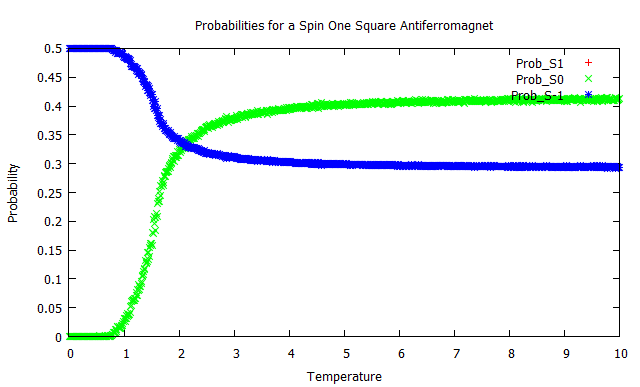
\includegraphics[scale=0.75]{Spin_1}
\caption{Probabilities for spin values of one, minus one
 and zero for a square spin one antiferromagnet using
Kawasaki dynamics.}
\label{Spin_1}
\end{center}
\end{figure}

\begin{figure}[h]
\begin{center}
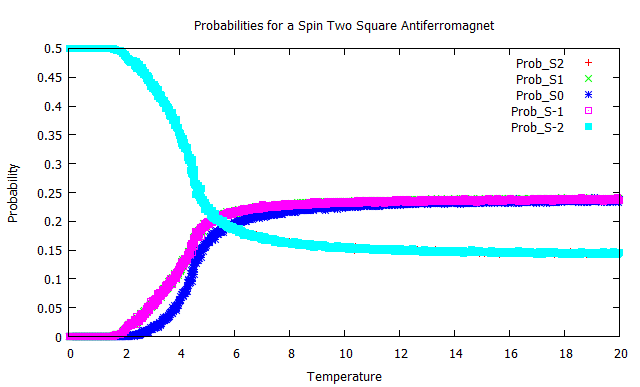
\includegraphics[scale=0.75]{Spin_2}
\caption{Probabilities for spin values of two, one, minus one, minus two and zero for a square spin two antiferromagnet using Kawasaki dynamics. Notice the rates at which the plus or minus one probabilites increase is faster than that for zero.}
\label{Spin_2}
\end{center}
\end{figure}

\begin{figure}[h]
\begin{center}
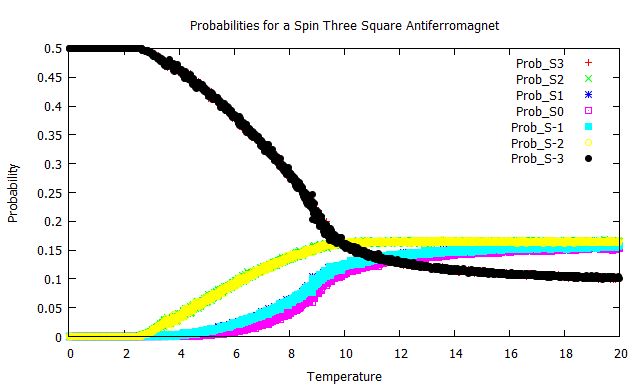
\includegraphics[scale=0.75]{Spin_3}
\caption{Probabilities for spin values of three, two, one, minus one, minus two, minus three and zero for a square spin three antiferromagnet using Kawasaki dynamics. Notice that the rate that the probabilities plus or minus two increase is faster than that of plus or minus one which is in turn faster than zero.}
\label{Spin_3}
\end{center}
\end{figure}

\begin{figure}
\begin{center}
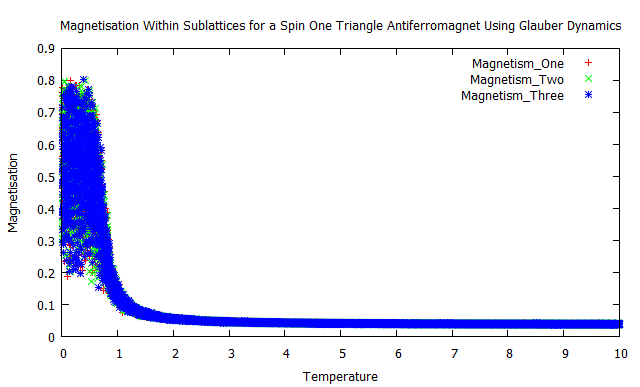
\includegraphics[scale=0.75]{Mag_G}
\caption{The magnetism for a cooling run using Glauber dynamics. Notice the lack of stability caused by the exchange of
sublattices below the critical point.}
\label{Mag_G}
\end{center}
\end{figure}

\begin{figure}
\begin{center}
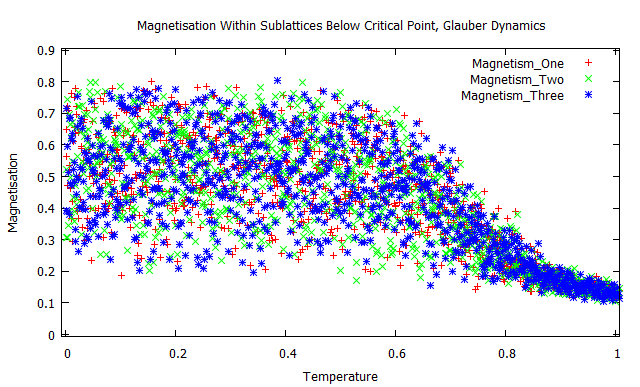
\includegraphics[scale=0.75]{Mag_G_BCP}
\caption{The magnetism for a cooling run, note that the exchange of sublattices occurs down to the zero temperature due to the lack of local stability, which allows the global stability to be removed at lower temperatures, despite the higher global stability of the kind of dynamics at higher temperatures compared to Kawasaki dynamics.}
\label{Mag_G_BCP}
\end{center}
\end{figure}

\begin{figure}
\begin{center}
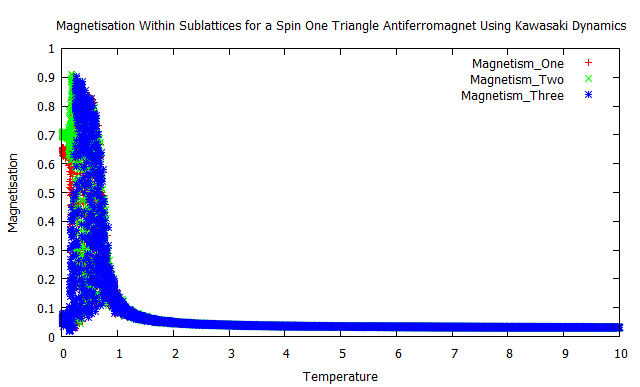
\includegraphics[scale=0.75]{Mag_K}
\caption{The magnetism for a cooling run using Kawasaki dynamics. Notice the lack of stability caused by the exchange of sublattices below the critical point.}
\label{Mag_K}
\end{center}
\end{figure}

\begin{figure}
\begin{center}
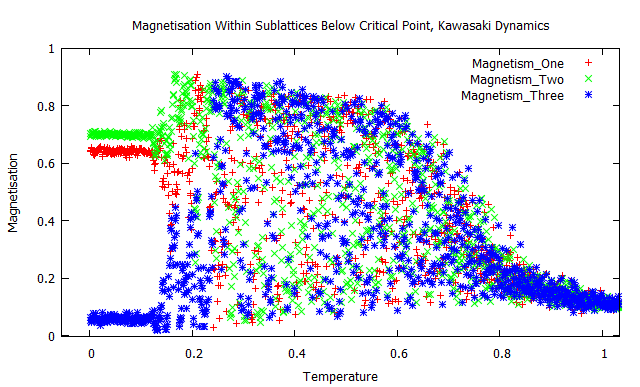
\includegraphics[scale=0.75]{Mag_K_BCP}
\caption{The magnetism for a cooling run, note that the exchange of sublattices freezes below a specific temperature due to the extra local stability given by Kawasaki dynamics. The overall magnetisations however do not represent the lowest energy state which would occur at $M_{1}=1$, $M_{2}=1$ and $M_{3}=0$ (these value can be exchanged).}
\label{Mag_K_BCP}
\end{center}
\end{figure}

\begin{figure}
\begin{center}
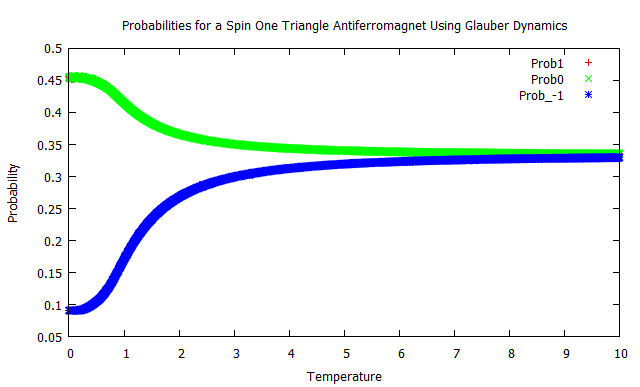
\includegraphics[scale=0.75]{Prob_G}
\caption{Probabilities for cooling the Glauber model. Although the probabilities come close to the lowest energy state values of $P_{1}=0.444$, $M_{-1}=0.444$ and $M_{0}=0.111$ the disorder in the magnetism implies that the model is merely forming pockets of stability with disordered walls between them.}
\label{Prob_G}
\end{center}
\end{figure}

\begin{figure}
\begin{center}
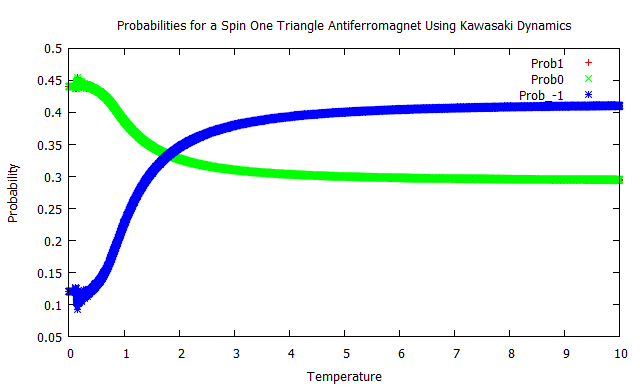
\includegraphics[scale=0.75]{Prob_K}
\caption{Probabilities for cooling the Glauber model. Although the probabilities come close to the lowest energy state values of $P_{1}=0.444$, $M_{-1}=0.444$ and $M_{0}=0.111$ the incorrect values in the magnetism implies that the model is merely forming pockets of stability with disordered walls between them.}
\label{Prob_K}
\end{center}
\end{figure}

\begin{figure}
\begin{center}
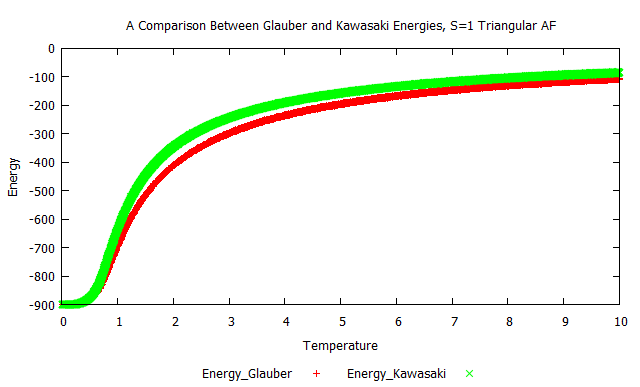
\includegraphics[scale=0.75]{Energy}
\caption{The energy curves for the model using Kawasaki and Glauber dynamics. Notice the steeper energy curve using Kawasaki model pointing to the models lower global stability, allowing it to disorder faster at the critical point.}
\label{Energy}
\end{center}
\end{figure}

\begin{figure}
\begin{center}
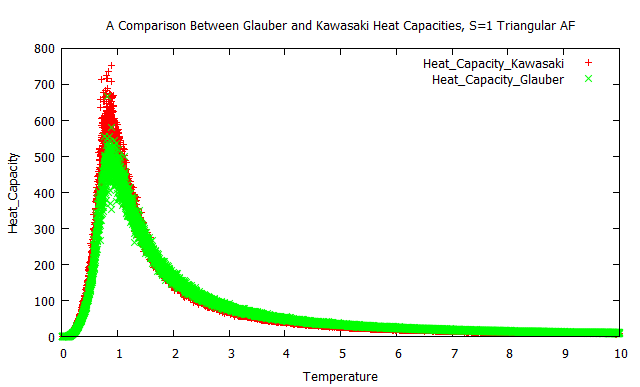
\includegraphics[scale=0.75]{Heat_Capacity}
\caption{The heat capacity curves for the model using Kawasaki and Glauber dynamics. Notice the much sharper heat capacity when using Kawasaki dynamics which results from the lower global stability caused by perturbing two lattices in one flip.}
\label{Heat_Capacity}
\end{center}
\end{figure}

\begin{figure}
\begin{center}
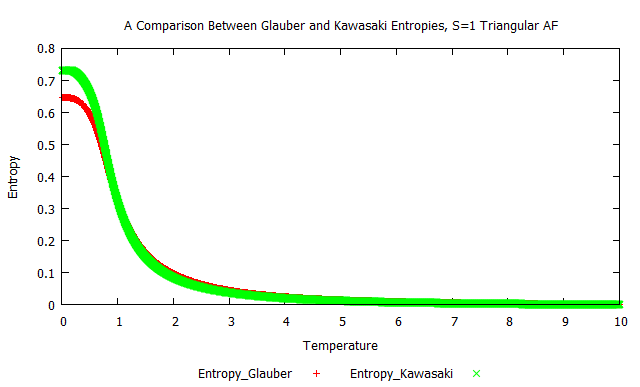
\includegraphics[scale=0.75]{Entropy}
\caption{The entropy curves for a cooling run. You can see that the Kawasaki dynamics give a higher entropy, due to the increased global instability below the critical point.}
\label{Entropy}
\end{center}
\end{figure}


\end{document}
